%%%%%%%%%%%%%%%%%%%%%%%%%%%%%%%%%%%%%%%%%%%%%%%%%%%%%%%%%%%%%%%
%
% Welcome to writeLaTeX --- just edit your LaTeX on the left,
% and we'll compile it for you on the right. If you give
% someone the link to this page, they can edit at the same
% time. See the help menu above for more info. Enjoy!
%
%%%%%%%%%%%%%%%%%%%%%%%%%%%%%%%%%%%%%%%%%%%%%%%%%%%%%%%%%%%%%%%

% --------------------------------------------------------------
% This is all preamble stuff that you don't have to worry about.
% Head down to where it says "Start here"
% --------------------------------------------------------------
 
\documentclass[12pt]{article}
 
\usepackage[margin=1in]{geometry}
\usepackage{amsmath,amsthm,amssymb}
\usepackage{enumitem}
\usepackage{cancel}

\setlist[enumerate,1]{label={(\alph*)}} %this changes enumerate to (a),(b),...

\usepackage{graphicx} %package to manage images

\newcommand{\A}{{\mathcal{A}}}
\newcommand{\C}{{\mathbb C}}
\newcommand{\CC}{{\mathcal{C}}}
\newcommand{\N}{{\mathbb N}}
\newcommand{\R}{{\mathbb R}}
\newcommand{\Q}{{\mathbb Q}}
\newcommand{\Z}{{\mathbb Z}}

\newcommand{\Aut}{{\rm Aut}}
\newcommand{\End}{{\rm End}}
\newcommand{\Hom}{{\rm Hom}}
\newcommand{\id}{{\rm id}}
\newcommand{\Ima}{{\rm Im}}
\newcommand{\Ker}{{\rm Ker}}
\newcommand{\Mor}{{\rm Mor}}
\newcommand{\Rad}{{\rm Rad}}
\newcommand{\Prob}{{\rm P}}

\renewcommand\labelitemi{-} %this changes itemize bullet points to dashes (-)

\usepackage{listings}
\usepackage{xcolor}

%New colors defined below
\definecolor{codegreen}{rgb}{0,0.6,0}
\definecolor{codegray}{rgb}{0.5,0.5,0.5}
\definecolor{codepurple}{rgb}{0.58,0,0.82}
\definecolor{backcolour}{rgb}{0.95,0.95,0.92}

%Code listing style named "mystyle"
\lstdefinestyle{mystyle}{
  backgroundcolor=\color{backcolour}, commentstyle=\color{codegreen},
  keywordstyle=\color{magenta},
  numberstyle=\tiny\color{codegray},
  stringstyle=\color{codepurple},
  basicstyle=\ttfamily\footnotesize,
  breakatwhitespace=false,         
  breaklines=true,                 
  captionpos=b,                    
  keepspaces=true,                 
  numbers=left,                    
  numbersep=5pt,                  
  showspaces=false,                
  showstringspaces=false,
  showtabs=false,                  
  tabsize=2
}

%"mystyle" code listing set
\lstset{style=mystyle}
 
\newenvironment{theorem}[2][Theorem]{\begin{trivlist}
\item[\hskip \labelsep {\bfseries #1}\hskip \labelsep {\bfseries #2.}]}
{\end{trivlist}}
\newenvironment{lemma}[2][Lemma]{\begin{trivlist}
\item[\hskip \labelsep {\bfseries #1}\hskip \labelsep {\bfseries #2.}]}
{\end{trivlist}}
\newenvironment{exercise}[2][Exercise]{\begin{trivlist}
\item[\hskip \labelsep {\bfseries #1}\hskip \labelsep {\bfseries #2.}]}
{\end{trivlist}}
\newenvironment{problem}[2][Problem]{\begin{trivlist}
\item[\hskip \labelsep {\bfseries #1}\hskip \labelsep {\bfseries #2.}]}
{\end{trivlist}}
\newenvironment{question}[2][Question]{\begin{trivlist}
\item[\hskip \labelsep {\bfseries #1}\hskip \labelsep {\bfseries #2.}]}
{\end{trivlist}}
\newenvironment{corollary}[2][Corollary]{\begin{trivlist}
\item[\hskip \labelsep {\bfseries #1}\hskip \labelsep {\bfseries #2.}]}
{\end{trivlist}}

\newenvironment{solution}{\begin{proof}[Solution]}{\end{proof}}
 
\begin{document}
 
% --------------------------------------------------------------
%                         Start here
% --------------------------------------------------------------
 
\title{Homework 2}%replace X with the appropriate number
\author{Mengxiang Jiang\\ %replace with your name
Stat 610 Distribution Theory} %if necessary, replace with your course title
 
\maketitle
 
\begin{problem}{1} %You can use theorem, exercise, problem, or question here.
  \textit{Statistical Inference} by Casella and Berger, 2nd Edition, Chapter 1, 
  Exercise 34.
  \begin{itemize}
    \item[34.] Two litters of a particular rodent species have been born,
    one with two brown-haired and one gray-haired (litter 1), and the other
    with three brown-haired and two gray-haired (litter 2). We select a
    litter at random and then select an offspring at random from the selected
    litter.
    \begin{enumerate}
      \item What is the probability that the animal chosen is brown-haired?
      \item Given that a brown-haired offspring was selected, what is the
      probability that the sampling was from litter 1?
    \end{enumerate}
    \begin{enumerate}
      \item Let $A$ be the event that the animal chosen is brown-haired,
      Let $B_i$ be the event that the sampling was from litter $i$, $i=1,2$.
      Then we have 
      \[
        \Prob(A) = \Prob(A|B_1)\Prob(B_1) + \Prob(A|B_2)\Prob(B_2) 
        = \frac{2}{3}\cdot\frac{1}{2} + \frac{3}{5}\cdot\frac{1}{2} 
        = \frac{19}{30}.
      \]
      \item By Bayes' theorem, we have
      \[
        \Prob(B_1|A) = \frac{\Prob(A|B_1)\Prob(B_1)}{\Prob(A)} 
        = \frac{\frac{2}{3}\cdot\frac{1}{2}}{\frac{19}{30}} 
        = \frac{5}{19}.
      \]
    \end{enumerate}
  \end{itemize}
\end{problem}

\begin{problem}{2}
  \begin{enumerate}
    \item Prove this alternative to Bayes' rule:
    \[
      \log\left(\frac{\Prob(A|B)}{\Prob(A^c|B)}\right)
      = \log\left(\frac{\Prob(A)}{\Prob(A^c)}\right)
      + \log\left(\frac{\Prob(B|A)}{\Prob(B|A^c)}\right).
    \]
    This expression is useful in genetics: conditional log odds of disease
    $(A)$ given gene $(B)$ = unconditional log odds of disease + log ratio
    of gene prevalence.
    \item Suppose $B_1,\dots,B_n$ are disjoint. Show that
    \[
      \Prob\left(B_j|\bigcup_{i=1}^n B_i\right) = \frac{\Prob(B_j)}
      {\sum_{i=1}^n \Prob(B_i)}. \quad \text{for each } j \in \{1,\dots,n\}.
    \]
  \end{enumerate}
  \begin{enumerate}
    \item By definition, we have
    \[
      \log\left(\frac{\Prob(A|B)}{\Prob(A^c|B)}\right)
      = \log\left(\frac{\frac{\Prob(A\cap B)}{\Prob(B)}}
      {\frac{\Prob(A^c\cap B)}{\Prob(B)}}\right)
      = \log\left(\frac{\Prob(A\cap B)}{\Prob(A^c\cap B)}\right).
    \]
    By the definition of conditional probability again and
    $\log(AB) = \log(A)+\log(B)$, we have
    \[
      \log\left(\frac{\Prob(A\cap B)}{\Prob(A^c\cap B)}\right)
      = \log\left(\frac{\Prob(A)\Prob(B|A)}{\Prob(A^c)\Prob(B|A^c)}\right)
      = \log\left(\frac{\Prob(A)}{\Prob(A^c)}\right)
      + \log\left(\frac{\Prob(B|A)}{\Prob(B|A^c)}\right).
    \]
    \item By definition, we have
    \[
      \Prob\left(B_j|\bigcup_{i=1}^n B_i\right)
      = \frac{\Prob\left(B_j \cap \bigcup_{i=1}^n B_i\right)}
      {\Prob\left(\bigcup_{i=1}^n B_i\right)}.
    \]
    Since $B_1,\dots,B_n$ are disjoint, we have
    \[
      \Prob\left(B_j \cap \bigcup_{i=1}^n B_i\right)
      = \Prob(B_j) \quad \text{and} \quad
      \Prob\left(\bigcup_{i=1}^n B_i\right)
      = \sum_{i=1}^n \Prob(B_i).
    \]
    Thus we have
    \[
      \Prob\left(B_j|\bigcup_{i=1}^n B_i\right)
      = \frac{\Prob(B_j)}{\sum_{i=1}^n \Prob(B_i)}.
    \]
  \end{enumerate}
\end{problem}

\begin{problem}{3}
  Yule's Paradox. A new drug is introduced to combat a disease. Let $R$ be
  the event that the drug is applied and $I$ be the event the patient improves.
  \begin{enumerate}
    \item Suppose the following proportions are reported, based on an
    experimental sample of patients.
    \begin{center}
      \begin{tabular}{|c|c c|c|}
        \hline
        & $R$ & $R^c$ &  \\
        \hline
        $I$ & 0.412 & 0.276 & 0.688 \\
        $I^c$ & 0.155 & 0.157 & 0.312 \\
        \hline
        & 0.567 & 0.433 & 1.000 \\
        \hline
      \end{tabular}
    \end{center}
    Find the chance the patient improves given that he takes the drug. Find
    the chance of improvement when he does not get the drug. What does this
    say about the efficacy of the drug?
    \item What the researchers \textit{did not} report is that patients
    can easily be categorized into two groups: those in the early stages of
    the disease $(E)$ and those not $(E^c)$. The proportions then become
    as follows.
    \begin{center}
      \begin{tabular}{|c|c c c c|}
        \hline
        & $E \cap R$ & $E \cap R^c$ & $E^c \cap R$ & $E^c \cap R^c$  \\
        \hline
        $I$ & 0.392 & 0.216 & 0.020 & 0.060 \\
        $I^c$ & 0.077 & 0.039 & 0.078 & 0.118 \\
        \hline
        & 0.469 & 0.255 & 0.098 & 0.178 \\
        \hline
      \end{tabular}
    \end{center}
    Now compare the chance of improvement with and without the drug just
    for the patients in the early stages. Do the same for the patients in
    the later stages. What do you think of the efficacy of the drug now?
    How should this experiment have been designed differently?
    (``Design'' here means ``number of patients chosen for each group
    in the study.'')
  \end{enumerate}
  \begin{enumerate}
    \item Let $A$ be the event that the patient improves.
    Then we have
    \[
      \Prob(A|R) = \frac{\Prob(A\cap R)}{\Prob(R)} = \frac{0.412}{0.567}
      \approx 0.7267, \quad
      \Prob(A|R^c) = \frac{\Prob(A\cap R^c)}{\Prob(R^c)} = \frac{0.276}{0.433}
      \approx 0.6374.
    \]
    Thus the chance of improvement is higher when the patient takes the drug.
    \item Let $E$ be the event that the patient is in the early stages of the
    disease. Then we have
    \[
      \Prob(A|E\cap R) = \frac{\Prob(A\cap E \cap R)}{\Prob(E \cap R)}
      = \frac{0.392}{0.469} \approx 0.8358
    \]
    \[
      \Prob(A|E\cap R^c) = \frac{\Prob(A\cap E \cap R^c)}{\Prob(E \cap R^c)}
      = \frac{0.216}{0.255} \approx 0.8471.
    \]
    Thus for patients in the early stages, the chance of improvement is
    slightly higher when the patient does not take the drug.\\
    Similarly, we have
    \[
      \Prob(A|E^c\cap R) = \frac{\Prob(A\cap E^c \cap R)}{\Prob(E^c \cap R)}
      = \frac{0.020}{0.098} \approx 0.2041
    \]
    \[
      \Prob(A|E^c\cap R^c) = \frac{\Prob(A\cap E^c \cap R^c)}{\Prob(E^c \cap R^c)}
      = \frac{0.060}{0.178} \approx 0.3371.
    \]
    Thus for patients in the later stages, the chance of improvement is
    higher when the patient does not take the drug.\\\\
    Based on the above results, it seems that the drug is not effective.\\\\
    The experiment should have been designed to have the same proportion
    of patients in the early stages and in the later stages for both
    groups (taking the drug and not taking the drug).
  \end{enumerate}
\end{problem}

\begin{problem}{4}
  Consider sampling with replacement from a population of size $N$ in which
  $M$ individuals would respond Yes (and $N-M$ would respond No).
  \begin{enumerate}
    \item Show that the first and second responses are independent. 
    As the responses are binary, it suffices to show that events
    $A_i = \{\text{``$i$-th response is Yes"}\}$, are independent, $i=1,2$.
    \item Show that the $n$ responses for a sample of size $n$ are
    \textit{mutually} independent. As in part (a), you can simply show that
    $A_1,\dots,A_n$ are mutually independent.
  \end{enumerate}
  \begin{enumerate}
    \item We have
    \[
      \Prob(A_1) = \frac{M}{N}, \quad \Prob(A_2) = \frac{M}{N}, \quad
      \Prob(A_1 \cap A_2) = \frac{M}{N} \cdot \frac{M}{N} = \Prob(A_1)\Prob(A_2).
    \]
    Thus $A_1$ and $A_2$ are independent.
    \item For any $k$ events $A_{i_1}, A_{i_2}, \dots, A_{i_k}$ where
    $1 \leq i_1 < i_2 < \dots < i_k \leq n$, we have
    \[
      \Prob(A_{i_1} \cap A_{i_2} \cap \dots \cap A_{i_k})
      = \left(\frac{M}{N}\right)^k
      = \Prob(A_{i_1})\Prob(A_{i_2})\cdots\Prob(A_{i_k}).
    \]
    Thus $A_1, A_2, \dots, A_n$ are mutually independent.
  \end{enumerate}
\end{problem}

\begin{problem}{5}
  Consider rolling two fair dice.
  \begin{enumerate}
    \item Define events $A = \text{``the first die is 6''}$,
    $B = \text{``the second die is 2''}$,
    $C = \text{``total of the dice is 7''}$. Are the events
    pairwise independent? Are they mutually independent?
    \item Now consider $A = \text{``the first die is even''}$,
    $B = \text{``the two dice are the same''}$,
    $C = \text{``total is 8, 9, or 10''}$. Are the events
    pairwise independent? Are they mutually independent?
    \item Suppose $A,B,C$ are \textit{pairwise} independent events,
    not necessarily mutually independent. Must $A$ be independent of
    $B \cap C$ or of $B \cup C$? Prove or show counterexamples.
  \end{enumerate}
  \begin{enumerate}
    \item We have
    \[
      \Prob(A) = \frac{1}{6}, \quad \Prob(B) = \frac{1}{6}, \quad
      \Prob(C) = \frac{1}{6}.
    \]
    \[
      \Prob(A \cap B) = \frac{1}{36} = \Prob(A)\Prob(B), \quad
      \Prob(A \cap C) = \frac{1}{36} = \Prob(A)\Prob(C), \quad
      \Prob(B \cap C) = \frac{1}{36} = \Prob(B)\Prob(C).
    \]
    Thus $A,B,C$ are pairwise independent. However, we have
    \[
      \Prob(A \cap B \cap C) = 0 \neq \Prob(A)\Prob(B)\Prob(C).
    \]
    Thus $A,B,C$ are not mutually independent.
    \item We have
    \[
      \Prob(A) = \frac{1}{2}, \quad \Prob(B) = \frac{1}{6}, \quad
      \Prob(C) = \frac{1}{3}.
    \]
    \[
      \Prob(A \cap B) = \frac{1}{12} = \Prob(A)\Prob(B), \quad
      \Prob(A \cap C) = \frac{1}{6} = \Prob(A)\Prob(C), \quad
      \Prob(B \cap C) = \frac{1}{18} = \Prob(B)\Prob(C).
    \]
    Thus $A,B,C$ are pairwise independent. However, we have
    \[
      \Prob(A \cap B \cap C) = \frac{1}{36} \neq \Prob(A)\Prob(B)\Prob(C).
    \]
    Thus $A,B,C$ are not mutually independent.
    \item No. Consider the following counterexample. Let
    $A = \{1,2\}, B = \{1,3\}, C = \{2,3\}$. Then we have
    \[
      \Prob(A) = \Prob(B) = \Prob(C) = \frac{1}{3}, \quad
      \Prob(A \cap B) = \Prob(A \cap C) = \Prob(B \cap C) = \frac{1}{6}.
    \]
    Thus $A,B,C$ are pairwise independent. However, we have
    \[
      \Prob(A \cap B \cap C) = 0 \neq \Prob(A)\Prob(B)\Prob(C).
    \]
    Thus $A,B,C$ are not mutually independent.\\
    Also, we have
    \[
      \Prob(A \cap (B \cap C)) = 0 \neq \Prob(A)\Prob(B \cap C),
    \]
    \[
      \Prob(A \cap (B \cup C)) = \frac{1}{3} \neq \Prob(A)\Prob(B \cup C).
    \]
    Thus $A$ is neither independent of $B \cap C$ nor of $B \cup C$.
  \end{enumerate}
\end{problem}

\begin{problem}{6}
  Two shaved dice are such that the chance of a 1 or 6 is 1/5 each,
  and the chance of a 2, 3, 4 or 5 is 3/20 each.
  \begin{enumerate}
    \item Find the chance of a total of 7 is obtained when the dice
    are rolled.
    \item Now suppose the dice are repeatedly rolled independently
    for a total of 6 times. Let $Y$ be the number of times that a total
    of 7 is obtained. Find the pmf and cdf of $Y$ and plot both.
    (A line graph works best for a pmf: draw a line or narrow bar of
    height $f_Y(x)$ at value $x$. Also, be sure to explicitly indicate
    the cdf's value at each of the jump points with, say, a small
    darkened circle.)
  \end{enumerate}
  \begin{enumerate}
    \item Let $A$ be the event that a total of 7 is obtained when the
    dice are rolled. Then we have
    \[
    \begin{aligned}
      \Prob(A) &= \Prob((1,6)) + \Prob((2,5)) + \Prob((3,4))
      + \Prob((4,3)) + \Prob((5,2)) + \Prob((6,1))\\
      &= 2\cdot\frac{1}{5}\cdot\frac{1}{5} + 2\cdot\frac{3}{20}\cdot\frac{3}{20}
      + 2\cdot\frac{3}{20}\cdot\frac{3}{20}\\ 
      &= \frac{17}{100}.
    \end{aligned}
    \]
    \item Since each roll is independent and the chance of a total of 7
    is $\frac{17}{100}$, we have
    \[
      Y \sim \text{Binomial}\left(n=6, p=\frac{17}{100}\right).
    \]
    Thus the pmf of $Y$ is given by
    \[
      f_Y(y) = \binom{6}{y}\left(\frac{17}{100}\right)^y
      \left(1-\frac{17}{100}\right)^{6-y}, \quad y=0,1,2,3,4,5,6.
    \]
    The cdf of $Y$ is given by
    \[
      F_Y(y) = \sum_{k=0}^{\lfloor y \rfloor} f_Y(k)
      = \sum_{k=0}^{\lfloor y \rfloor} \binom{6}{k}
      \left(\frac{17}{100}\right)^k
      \left(1-\frac{17}{100}\right)^{6-k}, \quad y \geq 0.
    \]
    The following are the plots of the pmf and cdf of $Y$.
    \begin{center}
      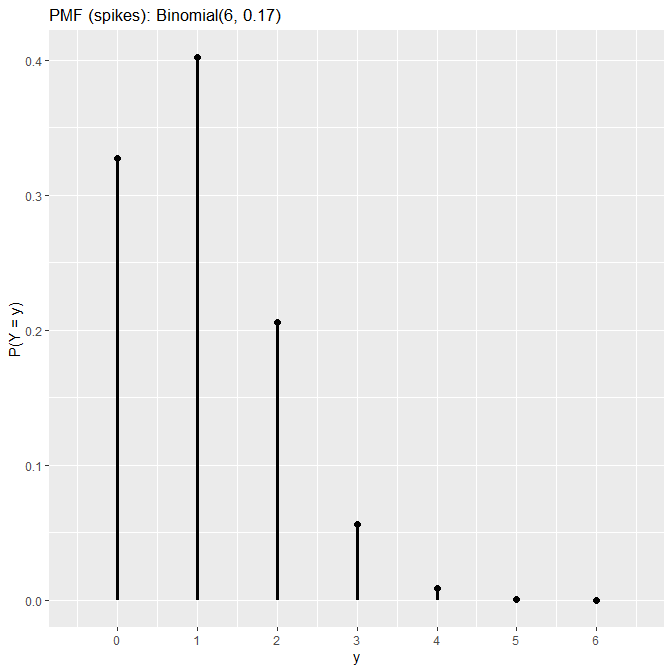
\includegraphics[width=\textwidth]{6pmf.png}
      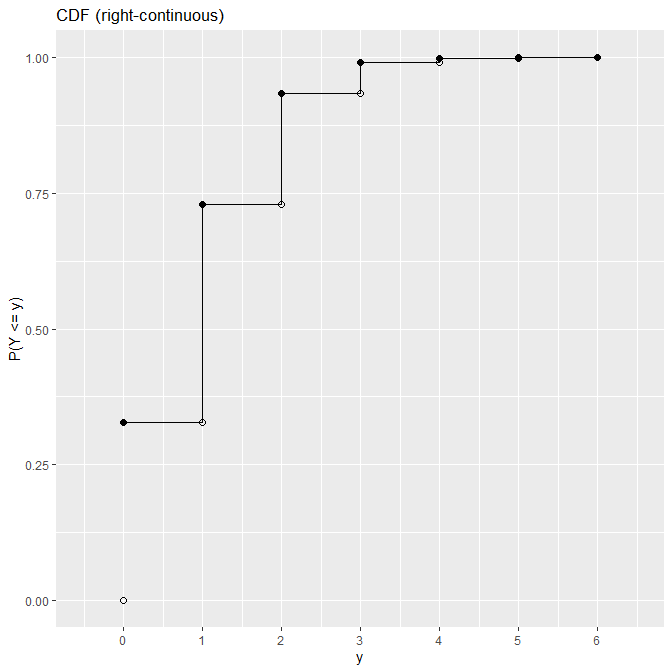
\includegraphics[width=\textwidth]{6cdf.png}
    \end{center}
  \end{enumerate}

\end{problem}

\begin{problem}{7}
  \textit{Statistical Inference} by Casella and Berger, 2nd Edition, Chapter 1, 
  Exercise 51.
  \begin{itemize}
    \item[51.] An appliance store receives a shipment of 30 microwave ovens,
    5 of which are (unknown to the manager) defective. The store manager
    selects 4 ovens at random, without replacement, and tests to see if they
    are defective. Let $X$ = number of defectives found. Calculate the pmf
    and cdf of $X$ and plot the pmf and cdf.
    \\\\
    The pmf of $X$ is given by
    \[
      f_X(x) = \frac{\binom{5}{x}\binom{25}{4-x}}{\binom{30}{4}}, \quad
      x=0,1,2,3,4.
    \]
    The cdf of $X$ is given by
    \[
      F_X(x) = \sum_{k=0}^{\lfloor x \rfloor} f_X(k)
      = \sum_{k=0}^{\lfloor x \rfloor} 
      \frac{\binom{5}{k}\binom{25}{4-k}}{\binom{30}{4}},
      \quad x \geq 0.
    \]
    The following are the plots of the pmf and cdf of $X$.
    \begin{center}
      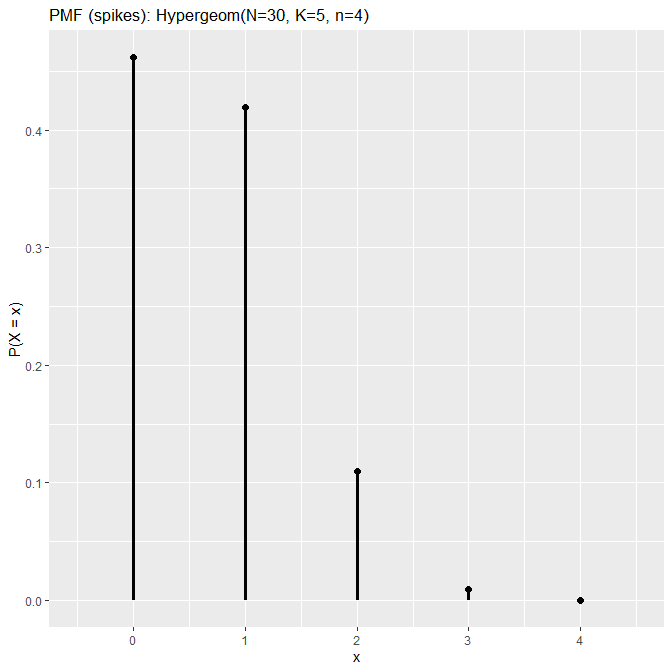
\includegraphics[width=\textwidth]{7pmf.png}
      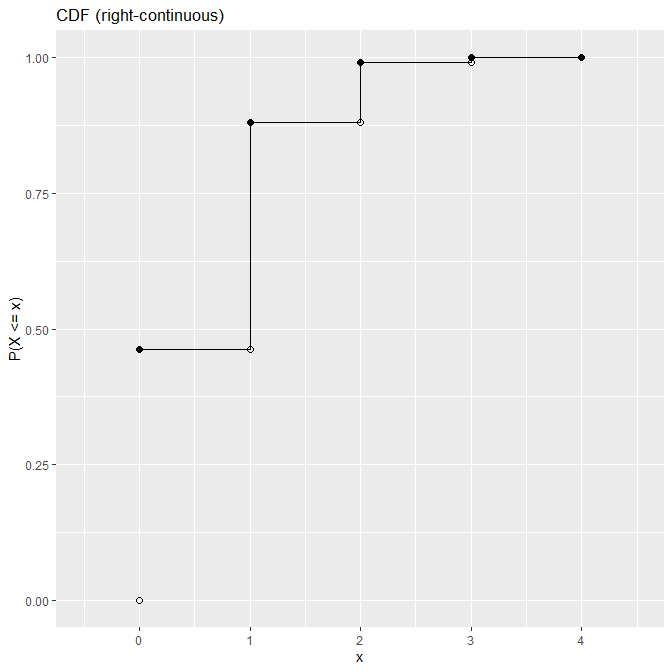
\includegraphics[width=\textwidth]{7cdf.png}
    \end{center}
  \end{itemize}
\end{problem}

\begin{problem}{8}
  Suppose $g(x) = 4\left(\frac{1}{3}\right)^x + \left(\frac{2}{3}\right)^x$
  for $x=1,2,\dots,$ and $g(x) = 0$ otherwise.
  \begin{enumerate}
    \item Find $c > 0$ such that $f(x) = cg(x)$ is a valid pmf.
    \item Find the corresponding cdf.
    \item Consider this game: A fair coin is flipped. If a Head appears
    then a fair die is rolled until either a 1 or a six appears. If a
    Tail is flipped then the die is rolled until a 2, 3, 4, or 5 appears.
    Let $X$ be the number of rolls and show that $f$ (the function in part
    (a)) is its pmf.
  \end{enumerate}
  \begin{enumerate}
    \item Since
    \[
      \sum_{x=1}^\infty g(x)=4\sum_{x=1}^\infty\!\left(\frac{1}{3}\right)^x
      +\sum_{x=1}^\infty\!\left(\frac{2}{3}\right)^x
      =4\cdot \frac{\frac{1}{3}}{1-\frac{1}{3}}+\frac{\frac{2}{3}}{1-\frac{2}{3}}
      =4\cdot\frac12+2=4,
    \]
    we need $c=\frac{1}{4}$ for $f = cg$ to be a pmf, since we need
    $\sum f = 1$.
    \item The cdf is
    \[
      F(x)=\sum_{k=1}^{\lfloor x\rfloor} f(k)
      =\frac{1}{2}\!\left(1-\left(\frac{1}{3}\right)^{\lfloor x\rfloor}\right)
      +\frac{1}{2}\!\left(1-\left(\frac{2}{3}\right)^{\lfloor x\rfloor}\right)
      =1-\frac12\!\left[\left(\frac{1}{3}\right)^{\lfloor x\rfloor}
      +\left(\frac{2}{3}\right)^{\lfloor x\rfloor}\right],
    \]
    with $F(x)=0$ for $x<1$. 
    \item We have
    \[
      \Prob(X=x|H)=\left(1-\frac26\right)^{x-1}\frac26
      =\left(\frac23\right)^{x-1}\left(\frac13\right)
      =\frac12\left(\frac23\right)^x,
    \]
    and
    \[
      \Prob(X=x|T)=\left(1-\frac46\right)^{x-1}\frac46
      =\left(\frac13\right)^{x-1}\left(\frac23\right)
      =2\left(\frac13\right)^x.
    \]
    With $\Prob(H)=\Prob(T)=\frac12$, we get
    \[
      \Prob(X=x)=\frac12\Prob(X=x|H)+\frac12\Prob(X=x|T)
      =\frac14\left(\frac23\right)^x+\left(\frac13\right)^x
      =f(x),\quad x=1,2,\dots
    \]
  \end{enumerate}
\end{problem}
% --------------------------------------------------------------
%     You don't have to mess with anything below this line.
% --------------------------------------------------------------
\end{document}
